\section{Introduction} 

\subsection{General Relativity and black holes}

General relativity, formulated by A. Einstein in 1915, is the current theory employed to describe gravity. According to this theory, gravity can be seen as a geometric property of a four-dimensional spacetime \cite{ferrari2020general}.

The curvature of spacetime is related to the matter and energy distribution within it, as described by the Einstein's Field Equations (EFEs):

\begin{equation}
G_{\mu\nu}={8\pi} \, T_{\mu\nu} \:,
\end{equation}

\noindent
where $G_{\mu\nu}$ is the Einstein tensor and $T_{\mu\nu}$ is the stress-energy tensor \cite{1916AnP...354..769E}, and we adopt the natural units, i.e. $ c=G=1$. 

A metric is mathematical object that describes the geometry of spacetime.
EFEs allow exact solutions which describe particular metrics. The simplest one was found by K. Schwarzschild, who describes an uncharged massive, non-rotating, spherically symmetric object. This solution correspond to a non spinning uncharged black hole (BH) \cite{1916SPAW.......189S}. Half century later, R. Kerr found a solution able to describe an uncharged spinning BHs \cite{1963PhRvL..11..237K}. 

BHs are extremely compact objects such as gravity is strong enough that not even light can escape from their event horizon.  
They can form as a consequence of stellar evolution: at the end of the life of a star, the internal pressure is no longer sufficient to counterbalance gravity and this lead to a gravitational collapse. The nature of the stellar remnants depends on initial mass: stars more massive than $\sim$ 20 $M _{\odot}$  \cite{1996A&A...305..871B}, will form BHs. 

BHs are classified in categories according to their masses \cite{article}:
\begin{itemize} 

\item stellar BHs, with  mass (M) $\in [5,100]  M _{\odot}$,
\item intermediate-mass BHs, with M $\in [10^2,10^5]  M _{\odot}$,
\item massive BHs, with M $\in [10^6,10^{11}]  M _{\odot}$;

\end{itemize}

\noindent
for this analysis we take into account only massive BHS.

The no-hair theorem states \cite{Tang_2022} that a BH is unequivocally characterized only by three parameters: mass, spin, and electric charge. The already presented  Schwarzschild and Kerr metrics describe uncharged BHs. There exist solutions able to describe charged BHs as, for example, the Reissner–Nordström metric \cite{1916AnP...355..106R} and Kerr–Newman metric \cite{adamo2016kerrnewman}. Respectively, they describe  non-rotating charged and rotating charged BHs. For this paper we neglect electric charged BHs, following the assumption that macroscopic astrophysical charged objects will rapidly be neutralized by surrounding plasma \cite{Teukolsky_2015}.


\subsection{Gravitational waves and merger of black holes}


In general relativity, a massive accelerating object changes the curvature of the spacetime: the perturbation propagates at the speed of light according to a wave equation, the so-called gravitational waves (GWs). BHs are powerful sources for this phenomena. 

The easiest mathematical description of a GW can be derived in the context of linearized gravity. This is an approximation of GR where the spacetime metric $ g_{\mu\nu} $ is the Minkowski flat metric $ \eta_{\mu\nu} $ plus a small deviation: 

\begin{equation}
g_{\mu\nu}=\eta_{\mu\nu} + h_{\mu\nu} \:, \quad \parallel h_{\mu\nu} \parallel \ll 1 \: .
\end{equation}

Under these assumptions, choosing a particular gauge condition, i.e. the Lorenz gauge  $\partial^\mu \bar{h}_{\mu\nu} = 0 $, one can linearize the EFEs:

\begin{equation}
 \Box \bar{h}_{\mu\nu} = -16\pi \, T_{\mu\nu}  \: 
\end{equation}

\noindent
where $ \bar{h}_{\mu\nu}$ is the  trace-reversed metric $ \bar{h}_{\mu\nu} = h_{\mu\nu} - \frac{1}{2} \eta_{\mu\nu} h $  \cite{Flanagan_2005}. 

In vacuum, $ T_{\mu\nu} = 0 $, the linearized EFEs admit a class of homogeneous solutions which are superpositions of plane waves:

\begin{equation}
 \bar{h}_{\mu\nu} = A_{\mu\nu} e^{i k_\alpha x^\alpha}  \: 
\end{equation}

\noindent
where 
\begin{itemize}
   \item \( A_{\mu\nu} \) is the wave amplitude,
    \item \( k^\alpha = (\omega, \mathbf{k}) \) is the wave four-vector,
    \item \( x^\alpha = (t, \mathbf{x}) \) represents the spacetime position.
\end{itemize}

The Lorenz gauge implies $ k^\mu A_{\mu\nu} = 0 $, in other words the wave amplitude is transverse to the wave vector \( k^\mu \). In order to remove unphysical degrees of freedom, we choose the \textit{Transverse-Traceless (TT) Gauge}. The transversality is already ensured by the Lorenz gauge, and we additionally impose $ A^\mu_{\ \mu} = 0 $. Now a GW is characterized only by two polarizations, denoted as $ h_{+} $ and $ h_ {\times}$, respectively \textit{plus} and \textit{cross} polarization \cite{Flanagan_2005}.

One of the main sources of GWs are Black-Hole Binaries (BHBs). A BH binary is a system composed by two BHs orbiting around each other. These systems can form in different ways, e.g. for stellar BH, in isolation at the end of the evolution of a massive star binary, or in a dense environment, such as dynamical interaction in star clusters \cite{Mapelli_2020}. About Massive Black-Hole Binaries (MBHBs), a BHB where the two BHs are both massive, their formation is not fully understood yet. It has been hypothesized that they are result of galaxy mergers. The massive BHs hosted at the center of such galaxies, reduce their separation through dynamical friction until they reach a distance of $\sim$ pc. At this stage, however, the efficiency of dynamical friction drops significantly, leading to what is known as the final parsec problem: the binary may stall at separations of the order of a pc, preventing further hardening and thus delaying or even inhibiting coalescence within a Hubble time. Various mechanisms have been proposed to overcome this stalling, such as interactions with gas, or the presence of a third massive object. This is still nowadays an open problems, future study of GWs have the aim to understand these mechanisms \cite{Milosavljevic__2003}.
 
Unlike to the Newtonian case, the system evolution is characterized by a loss of energy through the emission of GWs. We can identify three phases of the coalescence, visually represented in Fig. \ref{fig:IMR_introduction}:

\begin{itemize}
   \item \textit{Inspiral}: the two BHs orbit in quasi-circular orbits; the waveform of the GW is quasi-sinusoidal with increasing amplitude and frequency;
   \item \textit{Merger}: the two BHs plunge together and merge into a single distorted BH; the gravitational wave reaches its maximum amplitude;
   \item \textit{Ringdown}: the remnant BH settles into a stable Kerr configuration by emitting gravitational radiation in the form of damped oscillations, known as quasi-normal modes (QNMs).
\end{itemize}

\begin{figure}[h!]
    \centering
    \includegraphics[width=0.6\textwidth]{IMR_introduction.png}
    \caption{Typical shape of a GW signal generated by BHB where the three phases are highlighted. Credits to M. Favata, K. Thorne \cite{favata}. }
    \label{fig:IMR_introduction}
\end{figure}

In particular, QNMs are solutions of the Teukolsky equation \cite{zhao2022quasinormalmodesblack}, and according to the no-hair theorem they can only depend on the mass and the spin of the remnant BH. 
The study of QNMs (i.e. their frequencies and damping times) allow us to test the no-hair theorem, so the GR itself, this study field is called BH spectroscopy. On the other hand, the amount to which each mode is excited (i.e. its amplitude) and the relative phases between them do depend on the properties of the BHs in the binary and the binary dynamics \cite{Flanagan_1998, forteza2022novelringdownamplitudephaseconsistency}.
Due to these properties, a consistent model that incorporates both the merger-ringdown phase and the inspiral phase can enhance our ability to accurately measure the QNMs. This kind of waveforms are called Inspiral-Merger-Ringdown (IMR) waveform. We will focus on IMR waveform built according to the Effective-One-Body (EOB) formalism, as we will describe in \ref{ssec:Waveform_modelling}.


\subsection{Detection of gravitational waves and LISA}
\label{Detection_of_GWs}

GWs were originally described  by A. Einstein in 1916 but the first direct detection was only made on 14 September 2015 \cite{Abbott_2016}. This observation was made by LIGO interferometers and later on the Virgo one joined the observing run. These interferometers are based on the Michelson scheme, with two perpendicular arms of equal length at which end are placed two resonant masses. Fabry-Perot resonant cavities in the arms improve the interferometer sensitivity \cite{Accadia_2012, Aasi_2015}. The passage of GWs induces a variation in the arms length: 
\begin{equation}
	\delta L = hL \:,
\end{equation}

\noindent
where $ L $ is the arms length and $ h $ is the amplitude of the GW \cite{Accadia_2012}.

This variation produces a destructive interference that can be measured. Due to disturbance of seismic noise, ground-based interferometers, like LIGO and Virgo, are sensitive to GWs with frequencies higher than a few Hz \cite{Accadia_2012}. 
In particular, LIGO can detect GWs from sources in the frequency range from 10 Hz to 10 kHz, therefore the only compact object transient sources detected are stellar BHBs, neutron stars binaries and BH-neutron star binaries \cite{Martynov_2016}.
We refers to this kind of interferometer as ground-based, since they are located on the Earth.


A new kind of interferometer is being built to detect lower frequency sources, such as massive BHs mergers. Introducing LISA, Laser Interferometer Space Antenna, a space-based interferometer, which is scheduled to be launched in $\sim$ 2035, with a  mission duration of minimum 4 years.  LISA consists of three spacecrafts arranged in an equilateral triangle with each side measuring about 2.5 million kilometers. The proposed orbit for LISA is an Earth-trailing heliocentric orbit between 50 and 65 million km from Earth \cite{amaroseoane2017laserinterferometerspaceantenna}, as we can see schematically in Fig. \ref{fig:LISA_orbit}. 


\begin{figure}[h!]
    \centering
    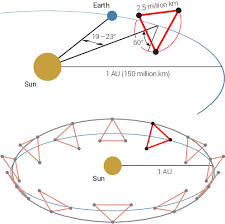
\includegraphics[width=0.4\textwidth]{LISA_orbit.png}
    \caption{Schematic representation of the Earth-trailing heliocentric orbit of LISA. Credits to \cite{amaroseoane2017laserinterferometerspaceantenna}. }
    \label{fig:LISA_orbit}
\end{figure}

The observatory will be based on three arms with six active laser working at  1064 nm, inside each spacecraft there are two free-fall test masses, one for each adjacent arm. Three independent interferometric combinations of the light travel time between the test masses are possible, allowing, in data processing on the ground, the synthesis of two virtual Michelson interferometers plus a third approximately null-stream, ideally containing no gravitational wave signal, used to identify instrumental noise or systematic errors \cite{amaroseoane2017laserinterferometerspaceantenna}.
The interferometers are all-sky monitors of GWs and do not require nor allow for any pointing towards specific sources. Regarding about frequency sensitivity regime, LISA is going to detect a huge variety of sources producing GWs in a range of [$10^{-4}-10^{-1}$] Hz \cite{amaroseoane2017laser}. This range will include:

\begin{itemize} 
\item MBHB,
\item extreme mass ratio inspiral (EMRI), the inspiral of a stellar mass compact object into a massive BH,
\item Galactic binaries, like white dwarf binaries,
\item potential signals from the early Universe.
\end{itemize}


The frequency gap between LIGO/Virgo and LISA will be partially explored by a future ground-based detector, the Einstein Telescope (ET), planned to work in the in $\sim$ 2040 \cite{abac2025scienceeinsteintelescope}.

Lower frequency GWs can be detected using a different technique such as Pulsar Timing Arrays (PTAs). A pulsar is a fast rotating neutron star, emitting a electromagnetic pulse in the radio wavelengths, making pulsars extremely precise clocks. PTAs makes use of the time delays in the arrival of radio pulses, caused by the passage of GWs \cite{Maiorano_2021}.




\subsection{Test of General Relativity}
\label{Test_of_GR}

The scientific method requires that a new theory must make testable predictions in order to be considered valid. This procedure has been followed for GR, with the first test proposed directly by Einstein himself in 1916 \cite{1916AnP...354..769E}. These test are commonly referred as the \textit{classical test of GR}, and are classified as kinematical tests as they involve the motion of a particle in a curved spacetime, in the weak-field limit. 

These classic tests are: 

\begin{itemize} 
\item \textit{Gravitational redshift of spectral lines:} the spectral lines of a light source, such as a star, are redshifted when observed from a region of weaker gravitational potential;

\item \textit{Light bending:} photons are massless particles so they follow null geodesics through spacetime. In the presence of mass or energy, spacetime is curved, and the path of light is deflected. As a result, the apparent position of a light source can appear displaced from its actual location — a phenomenon famously confirmed during the 1919 solar eclipse.

\item \textit{Periastron precession:} in GR, the orbits of massive particles around a spherically symmetric mass are not closed ellipses, as in Newtonian gravity. Instead, the point of closest approach, the periastron, advances slightly at each revolution. This explains, for example, the observed anomalous precession of Mercury’s perihelion. 
\end{itemize}

Alongside these tests, usually another kinematical one presented is the Shapiro time delay. This test was proposed only in 1964 by Irwin Shapiro, stating that, due to gravitational time dilatation, a signal takes longer time to travel in a curved region of the spacetime, rather than a flat region \cite{pössel2019shapirotimedelayequivalence}. The Shapiro time delay best constrain comes from measurement of radio signals between the Earth and the Cassini satellite, confirming the prediction of GR with an accuracy of 1 over $10^5$ \cite{Bertotti:2003rm}.


Different type of tests involves the emission of GW from non stationary sources in a strong-field regime. The first direct detection of a GW, as we discussed in \ref{Detection_of_GWs}, is itself a test of GR since it was possible to detect a phenomenological aspect not predicted by the Newtonian gravity. 

As discussed before, studying BH spectroscopy allows to test crucial prediction of GR, such as the no-hair theorem. The first detection, \textit{GW150914}, as been analysed under this aspect. The agreement between the postinspiral measurements of mass and spin and those using the full waveform supports the hypothesis that this merger produced a Kerr black hole, as predicted by GR \cite{Isi_2019}.

Even though GR has been successfully tested plenty of times in a variety of situation, this theory still has some intrinsic problems. For starters, GR is a classic physical theory, meaning it is fully deterministic and doesn't not include quantum mechanics at any level. Several attempts have been made to quantize GR without producing consistent and satisfying new theory \cite{wallace2000quantizationgravityintroduction}. 

Moreover GR has problems also from a cosmological point of view, leading to face the nature of dark matter (DM) and dark energy (DE). Multiple observations, e.g. the rotational curves of galaxies and gravitational lensing \cite{sofue2020rotationcurvemilkyway, article_Lensing}, strongly suggest the presence of a non baryonic matter, which interacts only trough gravity, leading to name it DM. These observations are in accordance with GR prediction if we include this new and exotic form of matter, but nowadays we only have candidates for the DM without explaining its nature. This induced the formulation of alternative theory to GR, i.e. MOND theories, which try to explain phenomenological observation without the requirement of DM \cite{klačka2020alternativeapproachgravitymond}.

Moving to the DE problem, from the EFEs is it possible to derive the Friedman equations under the assumptions of homogeneous and isotropic universe, which links the behaviour of the universe, such as its global geometry and its acceleration state, to its total matter-energy content. Solving these equations, the universe is not static but in expansion. Einstein did not believe in this implication and modify its equation by adding a term to the Einstein tensor, $ \Lambda g_{\mu\nu} $, trying to impose the static condition to the universe. Mathematically the solution it is not stable, and 1929 Edwin Hubble discovered that the universe is in expansion \cite{bagla2009hubblehubbleslawexpanding}, leading to discard the cosmological constant $ \Lambda$. At the end of the XX century, the discovery of the accelerated expansion of the universe \cite{Huterer_2017}, leads to a come back of the cosmological constant, which reflect the presence of a new kind of energy, the DE. The modified EFEs explains these phenomena but GR does not say what DE is, $\Lambda$ does not arise from first principles, and deriving $\Lambda$ as the vacuum energy from quantum field theory leads to a mismatch of 120 orders of magnitude with the value derived from observations.

All these open problems we listed, failed to be exhaustively explained by GR, are the reasons why researcher continue to test GR and trying to find evidence for theories beyond GR. Several new theories have been proposed to surpass GR, such as scalar-tensor theories or $f(R)$ gravity \cite{Naruko_2016, Sotiriou_2010}, but it is particularly difficult to test them. For instance, create a GW waveform from EFEs equation, to compare with observations, it's already extremely challenging and requires different assumptions to simply the problem. Following the same procedure for alternative theories is significantly harder. Due these difficulties, a new kind of test are worthy to be mentioned, the \textit{agnostic tests}.

An agnostic test refers to a method of testing a theory that doesn't make assumptions about the specific nature of any potential deviations from that theory. Instead, it probes for any deviation in a more general, model-independent way. This approach contrasts with \text{theory-specific} tests, which focus on the predictions of a particular alternative theory. As we anticipated, agnostic tests assume a crucial role in testing GR since theory-specific tests for alternative theories are not feasible for now. Moreover, it is reasonable to expect that any new theory extending GR will not differ radically from it, since GR already describes a vast array of astrophysical phenomena with remarkable accuracy. Between the types of agnostic test, in this paper we will focus on \textit{parameterized tests}, where we add parameterized deviations from GR in the waveform \cite{Carson_2021}, as we see in \ref{Test_of_GR_using_fractional_deviations}.

These tests will allow us to quantify the impact of systematic errors previously observed \cite{toubiana2024measuringsourcepropertiesquasinormalmode}, which arise due the inaccuracy of GW signal model. We will present a modified version of the signal model with the aim to absorb biases caused by systematics.
